\title{"Comparing Local Outlier Factor and Random Forest Algorithms for Anomaly Detection in Raw Water Quality"}
\documentclass[12pt]{report}
\usepackage[english]{babel}
\usepackage[utf8x]{inputenc}
\usepackage{listings}
\usepackage{amsmath}
\usepackage{graphicx}
\usepackage[colorinlistoftodos]{todonotes}
\usepackage{glossaries}
\usepackage{pdfpages}
\usepackage{acronym}
\usepackage{hyperref}
\usepackage{setspace}
\usepackage{times}

\graphicspath{./}

\makeglossaries

\newglossaryentry{DeKUT}
{
    name=DeKUT,
    description={Dedan Kimathi University of Technology}
}

\newglossaryentry{LOF}{name = LOF, description  = {Local Outlier Factor}}
\newglossaryentry{NYEWASCO}
{name = NYEWASCO, 
description  = {Nyeri Water and Sanitation Company } 
}

\newglossaryentry{IF}{name  = IF ,description  = {Isolated Forests } }
\newglossaryentry{RRCF}{name  = RRCF ,description  = {Robust
random cut forest}}


\begin{document}
\renewcommand{\bibname}{\centering REFERENCES}
\begin{titlepage}

	\centering
			
\includegraphics[width=0.5\textwidth]{dekut.png}
		
		\vspace{1cm}
		{\scshape\LARGE Dedan Kimathi University of Technology\par}
		\vspace{1cm}
		{\scshape\Large Bachelor of Science in Mathematics and Modeling Processes\par}
		\vspace{1.5cm}
		{\huge Comparing Local Outlier Factor and Random Forest Algorithms for Anomaly Detection in Raw Water Quality\par}
		\vspace{1cm}
		{\large\itshape NAME: KENNEDY WAMBUGU KINYUA\\REG: S084-01-2296/2021\par}
		\vfill
		\large \textbf{A research proposal submitted to the department of mathematics and physical science in partial fulfillment of requirement for award of the bachelor degree in bachelor of science in mathematics and modeling processes.}
\end{titlepage}


\linespread{1.5}
\pagenumbering{roman}
\begin{titlepage}
%\center
\Large \textbf{DECLARATION}\\[0.5cm]
\center 
\large DECLARATION BY THE STUDENT\\
%\large \textbf{Subject code} \\[0.5cm]
\paragraph{I declare that the work contained in this research proposal is my original work
and has not been presented for examination in any other University or
institution of higher learning.}

\begin{tabular}{p{0.4\linewidth}p{0.5\linewidth}}
  \textbf{Name: Kennedy wambugu kinyua} \\
  \vspace{12pt}
  signature: \dotfill & \vspace{12pt}  Date: \dotfill \\
\end{tabular}
\smallskip
%\left
\large DECLARATION BY THE SUPERVISOR\\
Department of Mathematics and Physical Sciences \\
\begin{tabular}{p{0.4\linewidth}p{0.5\linewidth}}
  \textbf{Name: MR. Rodgers  Amenya} \\
  \vspace{12pt}
  signature: \dotfill & \vspace{12pt}  Date: \dotfill \\
\end{tabular}
%\textbf{\large \today}
\end{titlepage}


%\newacronym{fpga}{FPGA}{Field Programmable Gate Array}
\newacronym{OSI}{OSI}{Open Standard Interface}
\newacronym{VHSIC}{VHSIC}{Very High Speed Integrated Circuit}
\newacronym{VHDL}{VHDL}{VHSIC Hardware Description Language}
\newacronym{VGA}{VGA}{Video Graphics Array}
\newacronym{bpp}{bpp}{bits per pixel}
\newacronym{TTL}{TTL}{Transistor Transistor Logic}
\newacronym{DTE}{DTE}{Data Terminal  Equipment}
\newacronym{DCE}{DCE}{Data Circuit Equipment}
\newacronym{USB}{USB}{Universal Serial  Bus}
\newacronym{UART}{UART}{Universal  Asynchronous Receiver/ Transmitter}
\newacronym{EIA}{EIA}{Electronic  Industries Alliance}
\newacronym{VDD}{VDD}{Voltage Drain Drain}
\newacronym{HSYNC}{HSYNC}{Horizontal Synchronization}
\newacronym{VSYNC}{VSYNC}{Vertical Synchronization}
\newacronym{IP}{IP}{Intellectual Property}
\newacronym{ISE}{ISE}{Integrated Synthesis Environment}
\newacronym{LSB}{LSB}{Least Significant Bit}
\newacronym{MSB}{MSB}{Most Significant Bit}
\newacronym{DAC}{DAC}{Digital to Analog Converter}
\newacronym{FIFO}{FIFO}{First In First Out}
\newacronym{LUT}{LUT}{Look Up Table}
\newacronym{ASIC}{ASIC}{Application Specific Integrated Chip}
\newacronym{IC}{IC}{Integrated Chip}
\newacronym{uart}{UART}{Universal Asynchronous Receiver and Transmitter}
\newacronym{RGB}{RGB}{Red Green Blue}
\newacronym{RAM}{RAM}{Random Access Memory}
\newacronym{XST}{XST}{Xilinx Synthesis Tool}
\newacronym{DDR SDRAM}{DDR SDRAM}{Double data rate synchronous dynamic random-access memory}
\newacronym{RTL}{RTL}{Register Transfer Language}

\subsection*{DEDICATION}
\addcontentsline{toc}{section}{DEDICATION}
\par
This Research Project is dedicated to my loving parents (Richard K. Wambugu \& Esther A. Kinyua) and siblings
for their moral support, financial assistance, encouragement, as well
as their self-denial and desire in ensuring that I succeed and to the
department of mathematics and physical sciences for enabling me
to pursue this course.
\par

\clearpage

\subsection*{ACKNOWLEDGEMENT}
\addcontentsline{toc}{section}{ACKNOWLEDGEMENT}
First and foremost, I would want to express my gratitude to the
Almighty for the wisdom, knowledge, and spirit of persistence He
has bestowed upon me during my academic journey. I would like
to convey my heartfelt appreciation to my supervisor, Mr. Rogers
Amenya, for his devotion and commitment to ensuring I complete
an excellent research project. Iam grateful for Center for Data
Science and Artificial Intelligence (DSAIL) in the Dedan Kimathi
University of Technology (DeKUT) team , their director Dr. Ciira
wa Maina, DeKUT and Nahshon Mokua Obiri ,for their mentorship,
inspiration, support with resources in my project from Nyeri Water
and Sanitation Company (NYEWASCO) water quality laboratory.
\clearpage

%\subsection*{Acknowledgment}
%\addcontentsline{toc}{section}{Acknowledgment}
%\par
%\clearpage

\renewcommand{\sectionname}{}
\renewcommand\thesection{\arabic{section}}
\subsection*{\centering ABSTRACT}
\par
The increased use of real-time water quality monitoring using
automated systems with sensors demands and makes it
possible to identify unexpected values in time. Anomalies are
brought by technical issues that are likely to prevent detection
of problematic data manually at the incoming data rate. Use of
machine learning approaches to detect anomalies for water
quality data is the main focus of this article. There is analysis
of three t machine learning anomaly detection
techniques: the local outlier factor, the isolation forest and robust random cut forest. A subset data collected from deployment of sensors in a water
treatment plant (Nyeri-Kenya) will used to carry out extensive
analysis of experiments of the afore-mentioned techniques;
for turbidity and pH parameters.
\addcontentsline{toc}{section}{ABSTRACT}
\clearpage

\tableofcontents
\addcontentsline{toc}{section}{Table of contents}
\clearpage
\section*{ACRONYMS \& SYMBOLS}
\addcontentsline{toc}{section}{ACRONYMS \& SYMBOLS}
%\begin*{itemize}
    \item \textbf{LOF}: Local Outlier  Factor
    \item  \textbf{RRCF}" Random Robust  Cut  Forest. 
    \item \textbf{IF} Isolation Forests.
    \item \textbf{DSAIL} Center  of  Data Science  and  Artificial Intelligence. 
    \item  \textbf{NYEWASCO}  Nyeri Water
and Sanitation Company. 
%\end{itemize}
\clearpage
%\listoftables
%\addcontentsline{toc}{section}{List of tables}
%\clearpage

%\listoffigures
%\addcontentsline{toc}{section}{List of Figures}
%\clearpage

%\printglossary[type=\acronymtype,title=List of Symbols and Acronym]
%\addcontentsline{toc}{section}{List of Symbols and Acronyms}

%\clearpage
%\subsection{Acronames}


%\clearpage
\begin


\pagenumbering{arabic}


\section{\centering CHAPTER ONE}
\subsection{\centering INTRODUCTION & BACKGROUND INFORMATION}
\par
The interaction between human activities and the environment yields diverse effects, significantly impacting human health. Particularly, the growth of numerous slums, poor sanitation, and post-mining effects have disproportionately affected developing countries, contributing to environmental deterioration. In response, global initiatives have been established to promote ecological sustainability through environmental monitoring programs. Notably, air quality monitoring systems have been implemented by governments and international organizations as part of this effort, with proposals for water quality monitoring systems, and advancements in animal tracking for environmental sustainability.

Water, a fundamental resource for life, covering over 70\% of the Earth's surface, is crucial for survival. However, ensuring water quality presents challenges due to its complex network comprising various interconnected components such as lakes, rivers, creeks, estuaries, and wetlands. Fluctuating pollution levels across these components pose difficulties in assessing water quality.

Water quality encompasses chemical, physical, biological, and other constituents that vary based on seasons and geographical locations. Environmental factors and human activities significantly influence water quality, with climate, geological, and hydrological factors being primary determinants. Human activities impact water quality extensively, affecting both human and environmental health. Hence, constant monitoring of water quality is essential for identifying and preventing contamination issues.
\par
Anomalies in water quality analysis, often caused by ecological phenomena like floods or rainfall, as well as human and technical errors, can lead to erroneous decisions and conclusions. These errors may stem from communication breakdowns between servers and sensor nodes, sensor probe contamination, equipment malfunctioning, among other factors.
This research proposal seeks to build upon these foundations by further investigating advanced anomaly detection techniques, leveraging emerging technologies in data science and artificial intelligence to enhance the accuracy and efficiency of water quality monitoring systems. By refining anomaly detection algorithms and incorporating real-time data analytics, the proposed research aims to contribute to the sustainable management of water resources and the protection of human and environmental health.
\subsection{STATEMENT OF THE PROBLEM}
\par
Traditional statistical methods for anomaly detection often fall short when dealing with high-dimensional, non-linear, and dynamic data streams. Machine learning algorithms, on the other hand, offer a powerful and flexible approach to tackle this challenge. By leveraging advanced techniques such as density-based methods, isolation forests, and ensemble models, machine learning algorithms can learn the intrinsic patterns and characteristics of normal data, enabling them to effectively distinguish anomalies from regular observations. However, the efficacy of these algorithms varies across different domains and data distributions, necessitating a comprehensive evaluation and comparison of their performance on real-world water quality datasets.
\par
The  machine learning anomaly detection algorithms: Local Outlier Factor (LOF), Isolation Forest (IF) and  (RRCF) Robust
random cut foress. These algorithms are evaluated on a subset of water quality data collected from a water treatment plant, focusing on two critical parameters: turbidity and pH. The aim is   to identify the most effective and efficient algorithm for detecting anomalies in real-time water quality data streams, taking into account factors such as accuracy, computational complexity, and scalability. By addressing this problem, the research contributes to the development of reliable and robust anomaly detection systems, enabling timely intervention and proactive maintenance in water quality monitoring applications.

\subsection{JUSTIFICATION}
\par
Water quality monitoring is a critical aspect of environmental protection and public health. The increasing deployment of automated sensor networks for real-time water quality monitoring generates vast amounts of data. However, the presence of anomalies or outliers in this data, caused by factors such as equipment malfunctions, environmental changes, or human errors, can lead to inaccurate analyses and flawed decision-making processes. Failing to detect and address these anomalies in a timely manner can have severe consequences, including potential health hazards and environmental degradation. Traditional statistical methods may not be sufficient for accurately identifying anomalies in complex, high-dimensional, and dynamic data streams. Therefore, there is a pressing need for robust and efficient machine learning algorithms that can learn the intrinsic patterns of normal data and effectively detect anomalies in real-time. The research paper addresses this crucial issue by conducting a comprehensive evaluation and comparison of four prominent machine learning anomaly detection algorithms on real-world water quality data. By identifying the most effective and efficient algorithm, the study contributes to the development of reliable anomaly detection systems, enabling timely intervention, proactive maintenance, and ultimately safeguarding water resources and public health.
\subsection{OBJECTIVES}
\subsubsection{Main objective}
\begin{itemize}
    \item By identifying the most effective and efficient algorithm, the study contributes to the development of reliable anomaly detection systems.
\end{itemize}
\subsubsection{Specific objective}
\begin{itemize}
    \item Evaluate and compare two ML anomaly detection algorithms (LOF, IF, RRCF) on real water quality data.
\item Identify the most effective and efficient algorithm for detecting anomalies in real-time water quality data.
\item  Provide valuable insights  to enhance  water  quality  management  procedures to guarantee the  security  of  water  sources.
\end{itemize}
\subsection{Assumptions}
\begin{enumerate}
    \item The data collected from sensors is accurate, reliable, and representative of the actual water conditions.
\item  The  results and conclusions drawn from the study can be generalized to similar water quality monitoring scenarios and datasets.
\item Optimal parameter settings for the algorithms can be determined effectively.
\end{enumerate}
\subsection{Limitations}
\begin{enumerate}
    \item Limitations in the computational resources necessary for deploying machine learning algorithms.
\item Presumptions established during data preprocessing and fine-tuning of algorithm parameters.
\item  How well the results can be used for other types of water quality monitoring and data.
\end{enumerate}

\subsection{Scope of the  study}
\begin{itemize}
    \item Evaluation of the LOF algorithm and Random Forest algorithms for anomaly detection in raw water quality data.
\item Comparison of different machine learning techniques for real-time monitoring of water contamination.
Optimization of algorithm parameters to enhance accuracy and efficiency in anomaly detection.
\item Contribution of insights to enhance water quality management practices and ensure the safety of water sources.
\end{itemize}

\clearpage

\section{\centering CHAPTER TWO}
\subsection{\centering LITERATURE REVIEW}
\par
\subsubsection{Machine learning for anomaly detection and process phase
classification to improve safety and maintenance activities(Elena Q,R. Patriarca (2020)}
The paper "Machine Learning for Anomaly Detection and Process Phase Classification in Industrial Processes" \cite{ml_paper1} introduces an innovative methodology that combines machine learning algorithms with process phase identification to enhance anomaly detection in industrial settings facing dynamic operational conditions. By addressing the limitations of traditional signal processing techniques in such environments, the study underscores the crucial role of domain experts in delineating normal and abnormal behavior boundaries and extracting valuable insights from complex data. Through a detailed case study in the pharmaceutical industry, the paper showcases the practical utility and effectiveness of the proposed approach, achieving impressive results in anomaly detection. The research not only emphasizes the importance of real-time implementation but also highlights the need for continuous algorithm parameter updates to adapt to changing industrial landscapes.

\subsubsection{An integrated data-driven framework for surface water quality anomaly detection and early warning (Jie LiuPeng WangPeng WangDexun Jiang(2019))}
\par
The paper "An integrated data-driven framework for surface water quality anomaly detection and early warning" \cite{paper2} focuses on the importance of detecting anomalies in surface water quality to prevent harmful compounds from spreading due to environmental spills or intentional releases into rivers. A data-driven framework is developed for early warning detection of surface water quality anomalies, crucial for addressing river pollution in advance. The framework combines a Bayesian autoregressive (BAR) model for predicting water quality variations and an Isolation Forest (IF) algorithm for anomaly detection. Firstly, the BAR model predicts water quality variations using Bayesian inference. Then, the IF algorithm identifies anomalies by analyzing prediction residuals. The framework is applied to analyze and detect surface water quality variations and anomalies in the Potomac River, West Virginia, USA. Comparative analysis with other methods and scenarios demonstrates that the integration framework not only improves anomaly detection accuracy but also enables quick response for emergency operations.
\subsubsection{Robust random cut
forest based anomaly detection on streams (S. Guha, N. Mishra, G. Roy and O. Schrijvers(2016))}
\par
In the paper "Robust Random Cut Forest Based Anomaly Detection On Streams," \cite{paper3} the authors delve into the realm of anomaly detection in dynamic data streams using random cut forests. By proposing a robust data structure to encapsulate the input stream and introducing a novel definition of non-parametric anomalies based on the impact of unseen points, the study sheds light on the intricate process of identifying anomalies in evolving data environments. The algorithm's ability to adapt efficiently to changes in the data stream, including corrections and updates, showcases its practical relevance in real-world scenarios. Overall, the research contributes significantly to the field of anomaly detection by offering a fresh perspective on model complexity and dynamic data structures, paving the way for enhanced anomaly detection methodologies in streaming data applications.
\subsubsection{OF: Iden-
tifying Density-Based Local Outliers (M. M. Breunig, H.-P. Kriegel, R. T. Ng and J. Sander(2000))}
The paper by Breunig et al\cite{paper4}. introduces the concept of the local outlier factor (LOF) for outlier detection in datasets, emphasizing the importance of considering the degree of outlyingness for each object rather than a binary outlier classification. Through a detailed analysis of LOF properties and experimental validation, the authors demonstrate the effectiveness of LOF in identifying local outliers that traditional methods may miss. They provide insights into the impact of parameters like MinPts on LOF values and offer practical guidelines for selecting appropriate values. Overall, the paper contributes a valuable perspective on outlier detection, showcasing the significance of a local approach in uncovering meaningful outliers in complex datasets.
\subsubsection{Anomaly Detection: A Survey (Varun Chandola, Arindam Banerjee, and Vipin Kumar(2007))}
In their comprehensive survey on anomaly detection \cite{paper5}, Chandola, Banerjee, and Kumar delve into the intricate challenges and diverse applications of identifying patterns that deviate from expected normal behavior. They highlight the complexity of defining normal regions and the evolving nature of anomalies, emphasizing the difficulty in distinguishing between noise and true anomalies. By categorizing techniques into six distinct groups and discussing unique assumptions underlying each approach, the authors offer a structured overview that expands upon existing works. Their exploration of complex anomalies in various domains sheds light on the gap between algorithmic research focusing on simple anomalies and the nuanced anomalies prevalent in real-world scenarios. This survey not only contributes a broad perspective on anomaly detection techniques but also provides valuable insights for future research and practical implementations.
\clearpage 

\section{\centering CHAPTER THREE}
\subsection{\centering RESEARCH METHODOLOGY}

\subsubsection{Data Collection}
\begin{itemize}
    \item \textbf{Data Collection}: Subset data collected from sensors deployed in a water treatment plant in Nyeri, Kenya.
\end{itemize}
\subsubsection{Model Selection: Anomaly Detection Algorithms}
\begin{enumerate}
  \item  \textbf{Local Outlier Factor Algorithm:}
  \par
 It  is an algorithm used for Unsupervised outlier detection. It produces an anomaly score that represents data points which are outliers in the data set.
\begin{figure}[h]
    %\centering
    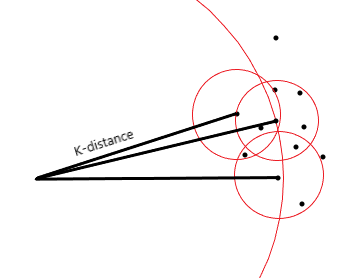
\includegraphics[width=0.5\linewidth]{lof.png}
    \caption{Local factor  algorithm k-distance}
    \label{fig:lof}
\end{figure}
\par
 This distance is used to calculate the reachability distance see figure \ref{fig:lof}. It is defined as the maximum of the distance between two points and the k-distance of that point.
\item  \textbf{Isolation Forest:}
\par
Isolation forest is a state-of-the-art anomaly detection algorithm which is very famous for its efficiency and simplicity see \ref{fig:iso}. By removing anomalies from a dataset using binary partitioning, it quickly identifies outliers with minimal computational overhead, making it the way to go for anomalies detection.
\begin{figure}[h]
    %\centering
    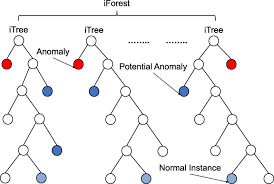
\includegraphics[width=0.5\textwidth]{iso.png}
    \caption{Isolation Forest}
    \label{fig:iso}
\end{figure}
\item \textbf{Robust
random cut forest:}
Robust Random Cut Forest (RRCF) algorithm is an ensemble method for detecting outliers in streaming data.
\end{enumerate}
\par
\begin{figure}[h]
    %\centering
    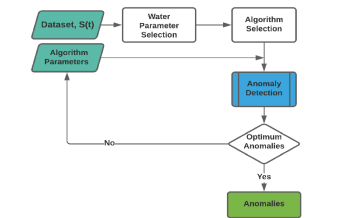
\includegraphics[width=0.5\textwidth]{methodology.png}
    \caption{Methodology}
    \label{fig:methods}
\end{figure}
\subsection{Expected  Outcome}
The anticipated results of the study include successful detection of anomalies in raw water quality data using the Local Outlier Factor (LOF) algorithm ,Isolation Forest (IF) and  Robust
random cut forest  (RRCF). The study aims to compare the performance of these algorithms in detecting outliers, optimize parameters for improved accuracy, assess feasibility for real-time monitoring, and contribute valuable insights to the field of water quality monitoring.
\newpage
\bibliographystyle{plainnat} % Changed plain to plainnat for references instead of bibliography
%\bibliography{refs}
\begin{thebibliography}{1}
\addcontentsline{toc}{section}{REFERENCES} % Changed Bibliography to REFERENCES
\bibitem{ml_paper1}
"Machine learning for anomaly detection and process phase classification to improve safety and maintenance activities" Elena Quatrini *, Francesco Costantino, Giulio Di Gravio, Riccardo Patriarca Department of Mechanical and Aerospace Engineering, University of Rome “La Sapienza”, Via Eudossiana, 18, 00184 Rome, Italy

\bibitem{paper2}
L. Jie, W. Peng, J. Dexun, N. Jun and Z. Weiyu, "An integrated data-driven framework for surface water quality anomaly detection and early warning," Journal of Cleaner Production, vol. 251, 2020. 
\bibitem{paper3}
 S. Guha, N. Mishra, G. Roy and O. Schrijvers, "Robust random cut forest based anomaly detection on streams," International conference on machine learning, pp. 2712-2721, 2016.
\bibitem{paper4}
] M. M. Breunig, H.-P. Kriegel, R. T. Ng and J. Sander, "LOF: Identifying Density-Based Local Outliers," Association for Computing Machinery, p. 93–104, 2000.
\bibitem{paper5}
Chandola V, Banerjee A, Kumar V. Anomaly Detection: A Survey. ACM Comput Surv 2009;41. https://doi.org/10.1145/1541880.1541882.\
\bibitem{paper6}
 H. Sahand, C. K. Matias and R. Brunner, "Extended Isolation Forest," IEEE Transactions on Knowledge and Data Engineering, pp. 1 - 1, 2019.
\bibitem{paper7}
M. Nahshon, W. M. Ciira and K. Henry, "A Raw Water Quality Monitoring System using Wireless Sensor Networks," International Journal of Computer Applications, vol. 174, no. 21, pp. 35-42, 2021.
%\end{itemize}
\end{thebibliography}


\clearpage
\end{document}
